\documentclass[12pt,letterpaper]{article}
\usepackage[utf8]{inputenc}
\usepackage[spanish]{babel}
\author{Las mil secciones son para no perderme durante la escritura}
\title{}
%\date{\today}
\date{}
%>>> Mate, símbolos
\usepackage{amsmath}
\usepackage{amssymb}
\usepackage{amsfonts}
\usepackage{mathtools}
\usepackage{newtxmath} % fuente?
\usepackage{array}
\usepackage{multirow} % tablas
\usepackage{tabularx} % tablas
%<<< Mate, símbolos
%>>> Bibliografía
\usepackage{csquotes} % citar
%\usepackage[backend=biber,style=alphabetic,sorting=nyt]{biblatex} % OVERLEAF
%\addbibresource{bibfile.bib} % OVERLEAF
\usepackage[backend=bibtex,style=alphabetic]{biblatex} % genérico no-overleaf
\usepackage{apacite}
%\bibliographystyle{apacite}
\bibliography{pro} % genérico no-overleaf
%>>>  Bibliografía
%>>> Imágenes
\usepackage{graphicx} % insertar
\usepackage{float} % ubicación flotante
%>>> Imágenes
%>>> Clickable hypers
\usepackage{hyperref}
\hypersetup{
    hyperindex=true,
    linktocpage=false,
    colorlinks=true,
    allcolors=black,
    bookmarksnumbered=true,
    unicode=true,
}
%<<< Clickable hypers
%>>> notas verticales QUITAR AL FINAL
%\usepackage{marginnote}
\usepackage{geometry}
\geometry{marginparwidth=.45cm,marginparsep=.45cm} %NO TOCAR EL PRIMER .45, constante
\newcommand{\notad}[1]{\normalmarginpar\marginpar{\rotatebox{90}{$\uparrow$ #1}}}
%
\newcommand{\notai}[1]{\reversemarginpar\marginpar{\rotatebox{90}{$\downarrow$ #1}}}
%
\newcommand{\notadhi}[1]{\normalmarginpar\marginpar{\rotatebox{270}{$\downarrow$ #1}}}
%
\newcommand{\notaihi}[1]{\reversemarginpar\marginpar{\rotatebox{270}{$\uparrow$ #1}}}
%<<< notas verticales QUITAR AL FINAL
%CIRCULOS
\usepackage{tikz}
\usetikzlibrary{shapes}
%%\usepackage[export]{adjustbox}
\usepackage{subcaption}
\usepackage{wasysym}
\usepackage{multicol}
%
%\usepackage[table]{xcolor}
\usepackage{microtype} %font kerning, poner atención
\usepackage{wrapfig}
\begin{document}
%\maketitle
%\renewcommand{\abstractname}{Resumen ejecutivo}\begin{abstract}
El uso de las redes sociales en el mundo ha generado la aparición de estudios enfocados a un sinnúmero de casos y aplicaciones. Estos estudios van siempre acompañados por técnicas de Procesamiento de Lenguaje Natural, unos más sofisticados y otros más básicos, a partir de palabras simples, considerando cierto tipo de personajes, considerando el uso de temas “hashtag”, en diferentes rangos de fechas, con enfoque de sentimientos, entre muchos otros casos. Pero de que sirve el Procesamiento de Lenguaje Natural sin un modelo estadístico que describa numéricamente lo que está sucediendo con las muestras de textos, como porque se dice algo repetidamente, o que hay en común en la opinión de la gente o de los reporteros, o cuál es la tendencia social y así sucesivamente. La estadística en esta propuesta de modelo tiene dos intervenciones. La primera es al inicio del proceso, con una estimación de lo que se pretende obtener y la segunda es con una comprobación de dicha estimación y en su caso una retroalimentación para asegurar ciertos valores usando aprendizaje de máquina y ajustando parámetros de categorización y diversificación de palabras, buscando confirmar o rechazar una suposición, con elementos numéricos bien fundamentados.
\end{abstract}

\tableofcontents
\pagebreak
\section {Marco teórico}\label{sec:marcot}
\subsection {Álgebra relacional}\label{subsec:algebra}Los cimientos del modelo relacional son el \emph{álgebra relacional}, las operaciones del álgebra producen nuevas relaciones, que pueden manipularse también por medio de operaciones del álgebra mismo. Una secuencia de operaciones de álgebra relacional forma una \emph{expresión de álgebra relacional} cuyo resultado es una relación que representa el resultado de una consulta (o solicitud de consulta) de base de datos. Estas operaciones pueden clasificar en dos grupos, operaciones de conjuntos*\notad{``set operations''} de la teoría de conjuntos matemáticos refiere a la operaciones \emph{UNION}, \emph{INTERSECTION}, \emph{SET DIFFERENCE} y \emph{CARTESIAN PRODUCT} (también llamado \emph{CROSS PRODUCT}). El otro grupo consiste en operaciones específicas para pases de batos relacionales: \emph{SELECT}, \emph{PROJECT} y \emph{JOIN}.

Se les puede clasificar también como operaciones \emph{unarias} o \emph{binarias} si estas operan en una o dos relaciones, respectivamente.

SELECT es una operación unaria denotada como
\begin{equation}
\sigma_\text{\textless condición de selección\textgreater}{\text{(R)}}
\end{equation}
Donde $\sigma$ denota el operador SELECT, y la condición de selección es una expresión booleana especificada en los atributos de la relación $R$. La condición de selección a su vez está formada de un número de clausulas en la forma
\begin{equation}
_\text{\textless nombre de atributo\textgreater\ \textless operador de comparación\textgreater\ \textless valor constante/nombre de atributo\textgreater}
\end{equation}
el \textless operador de comparación\textgreater\ normalmente un operador $\{=,<,\leq,>,\geq,\neq\}$.
\subsection {Modelo de base de datos relacional}\label{subsch:rdb}\section {Marco teórico}\label{sec:marco}
\subsection {Modelo relacional de base de datos}\label{subsec:rdb}
El \emph{modelo relacional de base de datos}, consiste en cinco componentes:
\begin{enumerate}
	\item Una colección de tipos escalares, pueden ser definidos por el sistema (INTEGER, CHAR, BOOLEAN, etc.) o por el usuario.
	\item Un generador de tipos de relaciones y un intérprete para las relaciones mismas.
	\item Estructuras para definir variables relacionales de los tipos generados.
	\item Un operador para asignar valores de relación a dichas variables.
	\item Una colección relacionalmente completa para obtener valores relacionales de otros valores relacionales mediante operadores relacionales genéricos.
\end{enumerate}
Aunque tersa esta lista es útil para delimitar lo que el modelo relacional es y no es.\\
Se debe comenzar definiendo los \emph{tipos}, ya que las relaciones se definen sobre ellos, son ``en esencia un conjunto finito de valores nombrados\textemdash todos los valores posibles de alguna categoría específica(...)''\cite{date12}.

Los \emph{atributos} son pares ordenados de combinaciones atributo-nombre/tipo-nombre y una \emph{tupla} es un par ordenado de atributos.
El modelo relacional también soporta varios tipos de \emph{llaves}, que poseen las propiedades de unicidad, ninguna contiene dos tuplas distintas con el mismo valor e irreductibilidad, ningún subconjunto suyo es tiene unicidad.
%La llave foránea (\emph{FK}) es una combinación o set se atributos FK en una relación $r2$ tal que se requiere que cada valor FK sea igual a algún valor de alguna llave K en alguna relación $r1$ ($r1$ y $r2$ no son necesariamente distintos).
\begin{table}[H]\centering\begin{tabular}{rc|c|c|l}
		\cline{2-4}
		\multicolumn{1}{r}{$\text{Atributos}\begin{cases}\ \end{cases}$}&\multicolumn{1}{|c|}{código}&\multicolumn{1}{c|}{fecha}&\multicolumn{1}{c|}{estado}&\multicolumn{1}{l}{}\\
		\cline{2-4}
		\multirow{3}{*}{$\text{Tuplas}\begin{cases}\\\\\end{cases}$}&\multicolumn{1}{|c|}{MX01}& 29-07-99&1&\multicolumn{1}{ l }{}\\
		\cline{2-4}
		&\multicolumn{1}{|c|}{MX02}&30-07-99&1&\multicolumn{1}{ l }{}\\
		\cline{2-4}
		&\multicolumn{1}{|c|}{MX03}&31-07-99&0&\multicolumn{1}{ l }{}\\
		\cline{2-4}
	\end{tabular}\caption{Representación de una tabla de una base en datos, la fila superior muestra tres atributos distintos y \emph{cada una} de las filas siguientes es una tupla.}\label{table:tupla}\end{table}
La \emph{restricción de integridad} (\emph{constraint}) es una expresión booleana que debe evaluarse como verdadera. Los \emph{constraints de tipo} definen los valores que constituyen un tipo dado y los \emph{constraints de base de datos} limitan los valores que pueden aparecer en cierta base de datos. Las bases de datos suelen tener múltiples constraints específicos, expresados en términos de sus relaciones, sin embargo, el modelo relacional incluye dos constraints genéricos, que aplican a cada base de datos:
\begin{itemize}
	\item Regla de integridad de identidad: Las \emph{llaves primarias} (\emph{PK}) deben ser no nulas.
	\item Regla de integridad de referencia: Las \emph{llaves foráneas} (\emph{FK}) deben tener relación (si $B$ referencia a $A$, $A$ debe existir).
\end{itemize}

Las operaciones del modelo relacional están cimientadas en el \emph{álgebra relacional}, las operaciones primitivas del álgebra producen nuevas relaciones, que pueden manipularse también por medio de operaciones del álgebra mismo. Una secuencia de operaciones de álgebra relacional forma una \emph{expresión de álgebra relacional} cuyo resultado es una relación que representa el resultado de una consulta (o solicitud de consulta) de base de datos.\cite{elma11} Estas operaciones pueden clasificar en dos grupos, operaciones de conjuntos*\notadhi{(así se llaman? checar libro en l'espagnol)``set operations''} de la teoría de conjuntos matemáticos refiere a la operaciones \emph{UNION}, \emph{INTERSECTION}, \emph{SET DIFFERENCE} (\emph{MINUS}) y \emph{CARTESIAN PRODUCT} (\emph{CROSS PRODUCT}). El otro grupo consiste en operaciones específicas para bases de datos relacionales: \emph{JOIN}, \emph{SELECT} y \emph{PROJECT}. Estas dos últimas, por operar con una sola relación, son también conocidas como \emph{operaciones unarias}.

SELECT elige un subconjunto de tuplas de una relación que satisfacen la condición de selección
\begin{equation}
\sigma_\text{\textless condición de selección\textgreater}{\text{(R)}}
\end{equation}
donde $\sigma$ denota el operador SELECT, y la condición de selección es una expresión booleana especificada en los atributos de la relación $R$.

PROJECT produce una nueva relación de atributos y tuplas*\notaihi{se explican hasta modelo rel, en los libros se explica primero} duplicadas
\begin{equation}
\pi_\text{\textless lista de atributos\textgreater}{\text{(R)}}
\end{equation}
donde $\pi$ es el denota el operador PROJECT y la lista de atributos es la sublista de atributos deseados de la relación $R$.

Las operaciones con dos relaciones reciben el nombre de \emph{operaciones binarias}. Si las relaciones $R(A_1,A_2,\ldots,A_n)$ y $S(B_1,B_2,\ldots,B_n)$ son compatibles de unión (tienen el mismo grado $n$ y $dom(A_i)=dom(B_i)$ para $1\leq i\leq n$) podemos usarlas para definir las siguientes operaciones binarias:
\begin{itemize}
	\item UNION: El resultado de esta operación se denota $R \cup S$, es una relación que incluye todas las tuplas que están en $R$, $S$ o ambos, se eliminan duplicados.
	\item INTERSECTION: El resultado de esta operación se denota $R \cap S$, es una relación que incluye todas las tuplas que están en ambos $R$ y $S$.
	\item SET DIFFERENCE: El resultado de esta operación se denota $R - S$, es una relación que incluye todas las tuplas que están en ambos $R$ pero no en $S$.
\end{itemize}

El operador CARTESIAN PRODUCT, denotado $R \times S$ es la operación binaria que no requiere compatibilidad de unión y produce un nuevo elemento al combinar cada miembro (tupla) de cada relación conjunto) con cada otro miembro de la otra relación. El resultado de $R(A_1,A_2,\ldots,A_n)$ y $S(B_1,B_2,\ldots,B_m)$ es una relación $Q$ con atributos $Q(A_1,A_2,\ldots,A_n,B_1,B_2,\ldots,B_m)$ (en ese orden) de grado $n+m$. El resultado $Q$ tiene una tupla por cada combinación de tuplas de $R$ y $S$.

JOIN $\Join$, es el operador utilizado para combinar tuplas relacionadas de dos relaciones en una sola tupla. Pertinente para procesar relaciones entre relaciones. Si tenemos dos relaciones $R(A_1,A_2,\ldots,A_n)$ y $S(B_1,B_2,\ldots,B_m)$ podemos escribir la operación JOIN como
\begin{equation}
R\Join_\text{\textless condiciones de unión\textgreater}S
\end{equation}
el resultado de la unión es la relación $Q$ con atributos $Q(A_1,A_2,\ldots,A_n,B_1,B_2,\ldots,B_m)$ (en ese orden). El resultado $Q$ tiene una tupla por cada combinación de tuplas de $R$ y $S$ que satisfacen las condiciones de unión.
\subsection {Inteligencia artificial}\label{subsec:intela}\emph{Inteligencia artificial} es definida como ``el esfuerzo por automatizar tareas intelectuales normalmente realizadas por humanos''\cite{cho18}, de este campo general se desprenden el \emph{aprendizaje maquinal} y el \emph{aprendizaje profundo}.
\subsection {Aprendizaje maquinal}\label{subsec:machinel}A diferencia del paradigma clásico de programación, donde los humanos introducen órdenes y datos para ser procesados de acuerdo con dichas reglas, en el aprendizaje maquinal el humano introduce datos y respuestas esperadas de estos datos ``y el producto son las reglas''*.\notad{``and out come the rules''}.

Tom Mitchel 97:
Se dice que un programa de computadora aprende de experiencia $E$ con respecto a una tarea $T$ y una medición de desempeño $P$, si su desempeño $T$, medido por $P$, mejora con experiencia $E$.

En vez de ser programado explícitamente, un sistema de aprendizaje maquinal es entrenado: se le presentan muchos ejemplos relevantes a una tarea, y si encuentra una estructura estadística en ellos, genera reglas para automatizar la tarea.
\subsection {Procesamiento de lenguaje natural}\label{subsec:nlp}El \emph{procesamiento de lenguaje natural}, es el conjunto de métodos para hacer accesible el lenguaje humano a las computadoras\cite{eise19}.*\notai{como que falta algo aquí?} Existen dos enfoques en lo que debe ser su tarea central: 
\begin{itemize}
    \item Entrenar sistemas de extremo a extremo*\notaihi{end-to-end, de principio a fin?} que transmuten texto sin procesar a cualquier estructura deseada.
    \item Transformar texto en una pila de estructuras lingüísticas de uso general que en teoría deben poder soportar cualquier aplicación.
\end{itemize}
Dos de los módulos básicos de NLP son \emph{búsqueda} y \emph{aprendizaje} con los que se puede resolver muchos problemas que podemos describir en la siguiente forma matemática
\begin{equation}
\begin{matrix}
\hat{y}=argmax\Psi(x,y;0),\\
y\in Y(x)
\end{matrix}
\end{equation}
donde,
\begin{itemize}
    \item $x$ es la entrada, un elemento de un conjunto $X$.
    \item $y$ es el resultado, un elemento de un conjunto $Y$.
    \item $\Psi$ es una función de puntuación (también conocida como \emph{modelo}), que va desde el conjunto $X\times Y$ hasta los números reales.
    \item $\emptyset$ es el vector de parámetros para $\Psi$.
    \item $\hat{y}$ es el resultado previsto, que es elegido para maximizar la función de puntuación.
\end{itemize}
El módulo de búsqueda se encarga de computar el $argmax$ de la función $\Psi$, es decir, encuentra el resultado $\hat{y}$ con la mejor puntuación con respecto a la entrada $x$. El módulo de aprendizaje encuentra los parámetros $\theta$ por medio del procesamiento de grandes conjuntos de datos de ejemplos etiquetados ${\{(x^i,y^i)\}}_{i=1}^{N}$.
\subsection {Regresión}\label{subsec:reg}Es común en el procesamiento de lenguaje natural utilizar \emph{modelos estadísticos lineales} para el modelado*\notad{modelo modelado?} del valor medio de una variable de resultado $Y$ como función de una independiente que pueden definirse con el modelo de \emph{regresión lineal simple}
\begin{equation}
E(Y)=\beta_0+\beta_1x
\end{equation}
en cambio, cuando se tiene más de una variable independiente se utiliza el modelo de \emph{regresión lineal múltiple}
\begin{equation}
E(Y)=\beta_0+\beta_1x+\ldots+\beta_kx_k
\end{equation}% nada de esto sirve
\subsection {Covarianza y correlación}\label{subsec:reg1}La covarianza mide qué tanto o tan poco las dos variables aleatorias cuyos valores esperados existen y son positivos tienen dependencia lineal, denotada $cov(X,Y)$ la covarianza de $X$ y $Y$ es definida como
\begin{equation}
cov(X,Y)=E[(X-EX)(Y-EY)]
\end{equation}
Cuando no se tiene una referencia para usar la covarianza, tiene sentido escalarla de acuerdo a la desviación estándar de las variables\cite{mat17}
\begin{equation}
p(X,Y)=\frac{cov(X,Y)}{\sqrt{var(X)}\sqrt{var(Y)}}
\end{equation}
denotada $corr(X,Y)$ de esta es la \emph{correlación} de $X$ y $Y$. Un coeficiente de relación $p = 0$ indica que no hay relación.
\subsection {Distribuciones}\label{subsec:dist}Blablabla distribuciones comunes para variables discretas:\cite{bala20}

SORT ME AND EXPLAIN

\begin{figure}[H]
\begin{subfigure}{.5\textwidth}\centering
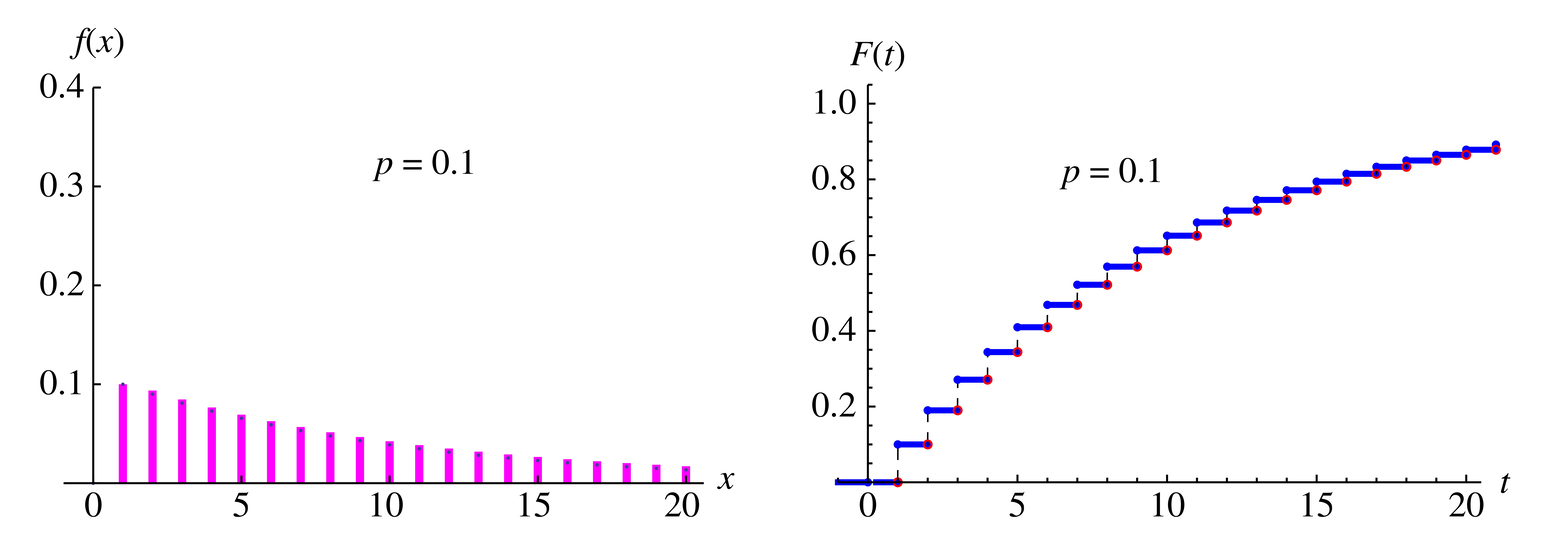
\includegraphics[width=.95\linewidth]{geom.png}
\caption{Geométrica}
\end{subfigure}\begin{subfigure}{.5\textwidth}\centering
\includegraphics[width=.95\linewidth]{binominal.png}
\caption{Binominal}
\end{subfigure}

\begin{subfigure}{.5\textwidth}\centering
\includegraphics[width=.95\linewidth]{negativabinominal.png}
\caption{Negativa binominal}
\end{subfigure}\begin{subfigure}{.5\textwidth}\centering
\includegraphics[width=.95\linewidth]{hyperg.png}
\caption{Hipergeométrica}
\end{subfigure}

\begin{subfigure}{.5\textwidth}\centering
\includegraphics[width=.95\linewidth]{gama.png}
\caption{$\Gamma$}
\end{subfigure}\begin{subfigure}{.5\textwidth}\centering
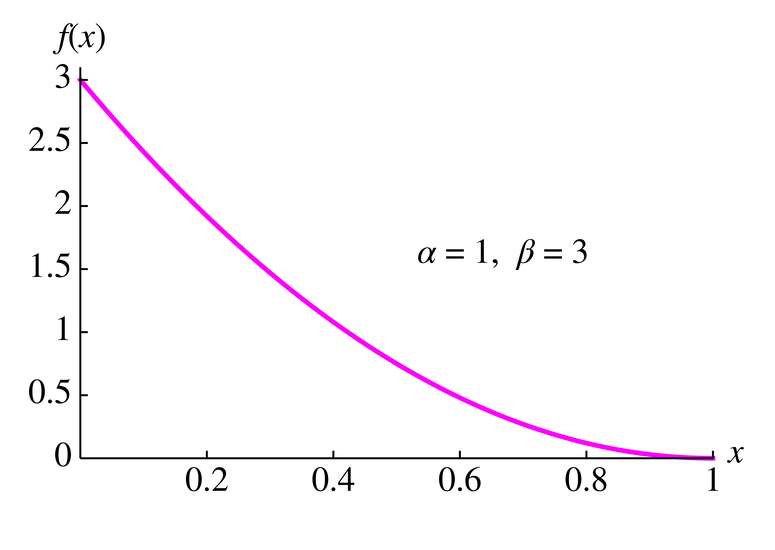
\includegraphics[width=.95\linewidth]{beta.png}
\caption{Beta}
\end{subfigure}

\begin{subfigure}{.5\textwidth}\centering
\includegraphics[width=.95\linewidth]{epsilon_lambda.png}
\caption{$\epsilon(\lambda)$}
\end{subfigure}\begin{subfigure}{.5\textwidth}\centering
\includegraphics[width=.95\linewidth]{normal.png}
\caption{Normal}
\end{subfigure}

\begin{subfigure}{.5\textwidth}\centering
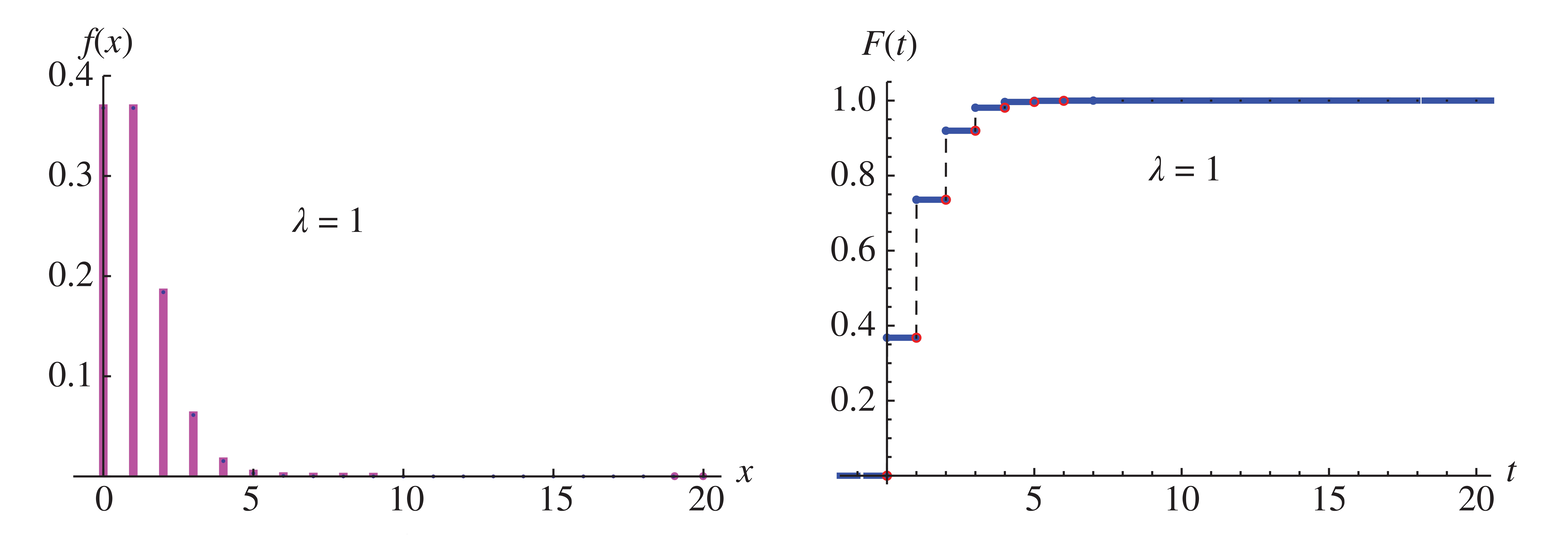
\includegraphics[width=.95\linewidth]{poisson.png}
\caption{Poisson}
\end{subfigure}\begin{subfigure}{.5\textwidth}\centering
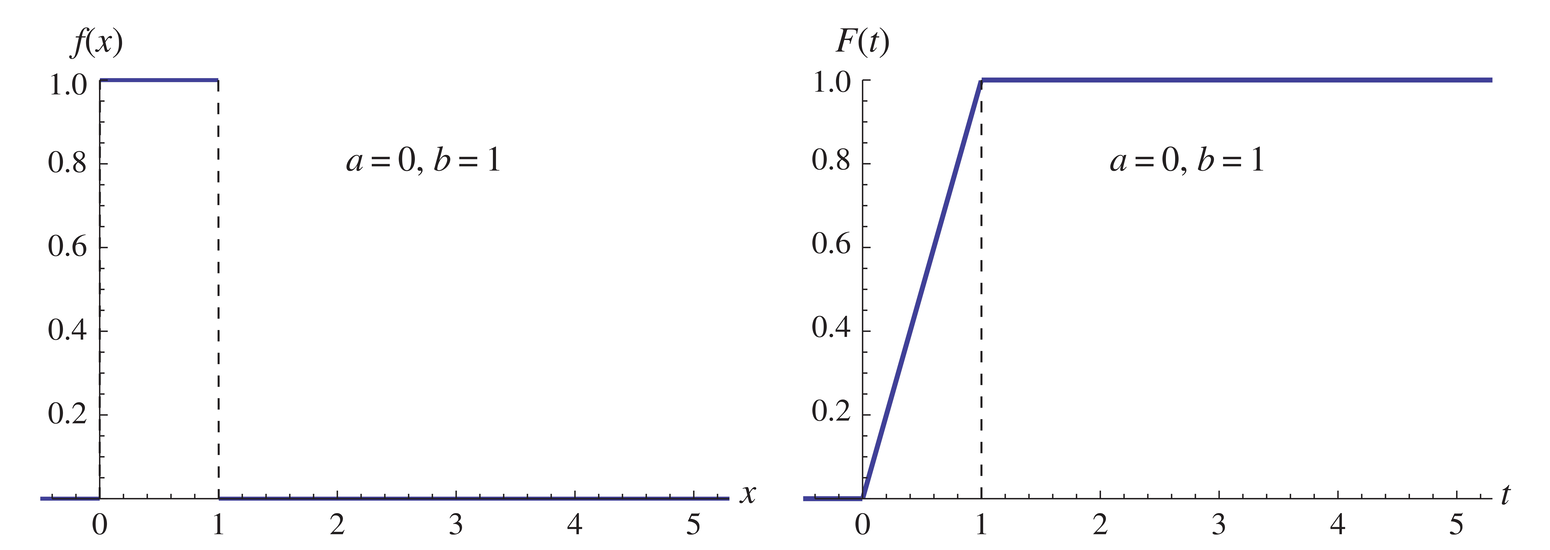
\includegraphics[width=.95\linewidth]{uniforme.png}
\caption{Uniforme}
\end{subfigure}
\end{figure}
\subsection {Probabilidad condicional}\label{subsec:pcond}El valor esperado de una suma de variables aleatorias es la suma de sus valores esperados individuales, este es el teorema de la \emph{linealidad del valor esperado}, donde para cada variable aleatoria $X,Y$ y cada constante $c$,
\begin{equation}
\begin{matrix}
E(X+Y)=E(X)+E(Y),\\
E(cX)=cE(X).
\end{matrix}
\end{equation}
\subsubsection {Binominal geométrica y negativa}
Distribución geométrica: Se tiene una secuencia de ensayos independientes Bernoulli, cada uno con la misma probabilidad de éxito $p\in(0,1)$, con ensayos realizados hasta que se alcanza el éxito. $X$ es el número de \emph{fallas} antes de la primera prueba exitosa por lo que $X$ tiene una \emph{distribución geométrica} con un parámetro $p$; denotado $X\sim Geom(p)$. Con esto podemos llegar a los teoremas de \emph{distribución geométrica de la función de probabilidad}, cuando $X\sim Geom(p)$, entonces la función de probabilidad de $X$ será
\begin{equation}
P(X=k)=q^kp
\end{equation}
para $k=1,2,\ldots,$ cuando $q=1-p$; y el teoremas de \emph{distribución geométrica de la función de distribución acumulativa}, cuando $X\sim Geom(p)$, entonces la función de distribución acumulativa de $X$ será
\begin{equation}
F(x)=
\begin{cases}
1-q^{\lfloor x\rfloor+1}, \text{ si } x\geq 0;\\
0, \text{ si }x < 0,
\end{cases}
\end{equation}
cuando $q=1-q$ y $\lfloor x\rfloor$ es el mayor entero y menor o igual a $x$.

El valor esperado geométrico de $X\sim Geom(p)$ es
\begin{equation}
E(X)=\sum_{k=0}^{\infty}kq^kp,
\end{equation}
cuando $q=1-p$. Aunque esta no es una serie geométrica, podemos llegar a ello
\begin{equation}\begin{matrix}
\sum_{k=0}^{\infty}q^k=\frac{1}{1-q}\\
\\
\sum_{k=0}^{\infty}kq^{k-1}=\frac{1}{{1-q}^2},
\end{matrix}
\end{equation}
finalmente multiplicamos ambos lados por $pq$, recuperando la suma original que queríamos encontrar
\begin{equation}
E(X)=\sum_{k=0}^{\infty}kq^kp=pq\sum_{k=0}^{\infty}kq^{k-1}=pq\frac{1}{{(1-q)}^2}=\frac{q}{p}.
\end{equation}
Primer valor esperado de éxito \emph{FS}, podemos definir a $Y\sim FS(p)$ como $Y=X+1$ donde $X\sim Geom(p)$, por lo que tenemos
\begin{equation}
E(Y)=E(X+1)=\frac{q}{p}+1=\frac{1}{p}.
\end{equation}

Las \emph{distribuciones binominales negativas} generalizan la distribución geométrica en lugar de esperar por un éxito, podemos esperar por cualquier número predeterminado $r$ de éxitos. En una secuencia de ensayos independientes Bernoulli con probabilidad de éxito $p$, si $X$ es el número de \emph{fallas} antes del éxito número $r$, entonces se dice que $X$tiene una distribución binominal negativa con parámetros $r$ y $p$, denotado $X\sim NBin(r,p)$.

La distribución binominal cuenta el número de éxitos en un número fijo de ensayos, mientras que la binominal negativa cuenta el número de fallas hasta alcanzar cierto número de éxitos. Si $X\sim NBin(r,p)$, entonces la función de probabilidad de $X$ es
\begin{equation}
P(X=n)=\binom{n+r-1}{r-1}p^rq^n
\end{equation}
para $n=0,1,2\ldots,$ donde $q=1=p$.
%\subsubsection{LOTUS}
%La \emph{ley del estadista inconsciente} (\emph{LOTUS}, por sus siglas en inglés) permite calcular $E(g(X))$ directamente usando la distribución de $X$, sin tener que encontrar la distribución de $g(X)$ primero: si $X$ es una variable discreta y $g$ es una función de $\mathbb{R}$ a $\mathbb{R}$, entonces
%\begin{equation}
%E(g(X))=\sum_{x}g(x)P(X=x),
%\end{equation}
%donde la suma se toma de todos los valores posibles de $X$. El valor esperado de $g(X)$ puede ser escrito en forma no agrupado como
%\begin{equation}
%E(g(X))=\sum_{s}g(X(s))p(\{s\}).
%\end{equation}
\subsubsection{Varianza, agregarlas a la secc que pertenecen}
Varianza de la geométrica (agregarla a la geom después de editar todo y hacerlo más breve)
\begin{equation}
Var(X)=E(X^2)-{(EX)}^2=\frac{q(1+q)}{p^2}-{(\frac{q}{p})}^2=\frac{q}{p^2}
\end{equation}
Varianza de la geométrica (lo mismo)
\begin{equation}
Var(X)=E(X^2)-{(EX)}^2=(n(n-1)p^2+np)-(np)^2=np(1-p).
\end{equation}

Una variable aleatoria $X$ tiene \emph{distribución de Poisson} (denotada $X\sim Pois(\lambda)$) con el parámetro $\lambda$, cuando $\lambda > 0$ si la PMF de $x$ es
\begin{equation}
P(X=k)=\frac{e^{-\lambda}\lambda^k}{k!}, k=0,1,2,\ldots.
\end{equation}
Varianza de la distribución de Poisson es
\begin{equation}
Var(X)=E(X^2)-{(EX)}^2=\lambda(1+\lambda)-\lambda^2=\lambda
\end{equation}
\subsubsection{r.v. continuas}
A diferencia de las variables discretas, las \emph{variables aleatorias continuas} pueden tomar cualquier valor real en un intervalo y tienen una \emph{distribución continua}. Para obtener la probabilidad deseadaWHOMST, se debe integrar la función de densidad de probabilidad sobre el rango apropiado
\begin{equation}
P(X\in A)=\int_{A}f(x)dx
\end{equation}
La distribución logística se obtiene
\begin{equation}
F(x)=\frac{e^x}{1+e^x}, x\in\Re
\end{equation}
El valor esperado de la continua función de distribución acumulada $f$ es
\begin{equation}
E(X)=\int_{-\infty}^{\infty}xf(x)dx
\end{equation}
la continua $U$ tiene dist unif en el intervalo $(a,b)$, denotada $U \sim Unif(a,b)$ si el área acumulada bajo la función de densidad de probabilidad es
\begin{equation}
f(x)=\begin{cases}
\frac{1}{b-a},\text{ si }a<x<b;\\
\text{de lo contrario, }0
\end{cases}
\end{equation}
$U \sim Unif(a,b)$ de una variable aleatoria es
\begin{equation}
\tilde{U}=a+(b-a)U
\end{equation}
Su varianza es
\begin{equation}
Var(U)=\frac{{(b-a)}^2}{12}
\end{equation}
La distribución normal ($X \sim N(\mu,\sigma^2)$)cuando $\mathbb{Z} \sim N(0,1)$ es
\begin{equation}
X=\mu+\sigma\mathbb{Z}
\end{equation}
Por lo tanto obtendremos el valor esperado de $\mu$ y varianza de $\sigma^2$
\begin{equation}
X=(\mu+\sigma\mathbb{Z})=E(\mu)+\sigma E(\mathbb{Z})=\mu
\end{equation}
\begin{equation}
Var=(\mu+\sigma\mathbb{Z})=Var(\sigma\mathbb{Z})=\sigma^2Var(\mathbb{Z})=\sigma^2.
\end{equation}

La \emph{distribución exponencial} de $X$ con un parámetro $\lambda$, cuando $\lambda>0$ si su función de densidad de probabilidad es $f(x)=\lambda e^{-\lambda x} , x>0$; denotada como $X \sim Expo(\lambda)$ es la siguiente
\begin{equation}
F(x)=1-e^{-\lambda x}, x>0
\end{equation}
\subsection {Variables aleatorias y sus distribuciones}\label{subsec:vayd}\subsubsection {Distribución de Bernoulli y binominal}
Una variable aleatoria tiene la \emph{distribución de Bernoulli} con un parámetro $p$ si $P(X=1)=p$ y $P(X=0=1-p)$, cuando $0<p<1$. Se escribe como $X \sim Bern(p)$, el símbolo $\sim$ significa ``distribuido como'' y la probabilidad $p$ es el \emph{parámetro}, que determina qué distribución de Bernoulli específica tenemos.

Supóngase que se realizan $n$ ensayos Bernoulli independientes, cada uno con probabilidad $p$ de éxito. $X$ sea el número de éxitos, la distribución $X$ se llama \emph{distribución binominal} con parámetros $n$ y $p$; se escribe $X \sim Bin(p,n)$.
$Bern(p)$ es la misma distribución que $Bin(1,p)$. Bernoulli es un caso especial de binominal, si $x \sim Bin(1,p)$, entonces la función de probabilidad de $X$ es
\begin{equation}
P(X=k)=\binom{n}{k}p^k(1-p)^{n-k}
\end{equation}
para $k=0,1,\ldots,n$ (y por otra parte $P(X=k)=0$).
\subsubsection {Distribución de hipergeométrica}
Si $X \sim HGeom(w,b,n)$, entonces la función de probabilidad de X es
\begin{equation}
P(X=k)=\frac{\binom{w}{k}\binom{b}{n-k}}{\binom{w+b}{n}},
\end{equation}
para enteros $k$ satisfaciendo $0\leq k\leq w$ y $0\leq n-k\leq b$, y $P(X=k)=0$. La estructura esencial de la distribución hipergeométrica se basa en que objetos en su población están clasificados usando dos tipos de etiquetas, al menos una de estas siendo asignada al azar.
Las distribuciones $HGeom(w,b,n)$ y $HGeom(n,w+b-n,1)$ son idénticas si $X$ y $Y$ tienen la misma distribución, podemos demostrarlo algebraicamente:
\begin{equation}
P(X=k)=\frac{\binom{w}{k}\binom{b}{n-k}}{\binom{w+b}{n}}=\frac{w!b!n!(w+b-n)!}{k!(w+b)!(w-k)!(n-k)!(b-n+k)!}
\end{equation}
\begin{equation}
P(X=k)=\frac{\binom{n}{k}\binom{w+b-n}{w-k}}{\binom{w+b}{w}}=\frac{w!b!n!(w+b-n)!}{k!(w+b)!(w-k)!(n-k)!(b-n+k)!}.
\end{equation}%if intro for bernolli and hyper neede, 3.4.6 has a bit a few useful lines
\subsubsection {Distribución uniforme discreta}
Teniendo $C$, un conjunto finito no vacío de números, se elige un número uniformemente al azar (o sea que todos los números tienen la misma posibilidad de ser elegidos), llámese $X$. Entonces se dice que $X$ una \emph{distribución uniforme discreta} con el parámetro $C$. Se dice entonces que la función de probabilidad de $X \sim DUNif(C)$ (la distribución uniforme discreta de $X$) es
\begin{equation}
P(X=x)=\frac{1}{|C|}
\end{equation}
para $x \in C$ (de lo contrario $0$) ya que la función de probabilidad debe sumar 1.
\subsection {Valor esperado}\label{subsec:valesp}%\subsubsection{LOTUS}
%La \emph{ley del estadista inconsciente} (\emph{LOTUS}, por sus siglas en inglés) permite calcular $E(g(X))$ directamente usando la distribución de $X$, sin tener que encontrar la distribución de $g(X)$ primero: si $X$ es una variable discreta y $g$ es una función de $\mathbb{R}$ a $\mathbb{R}$, entonces
%\begin{equation}
%E(g(X))=\sum_{x}g(x)P(X=x),
%\end{equation}
%donde la suma se toma de todos los valores posibles de $X$. El valor esperado de $g(X)$ puede ser escrito en forma no agrupado como
%\begin{equation}
%E(g(X))=\sum_{s}g(X(s))p(\{s\}).
%\end{equation}
%\subsubsection{Varianza, agregarlas a la secc que pertenecen}
%Varianza de la geométrica (agregarla a la geom después de editar todo y hacerlo más breve)
%\begin{equation}
%Var(X)=E(X^2)-{(EX)}^2=\frac{q(1+q)}{p^2}-{(\frac{q}{p})}^2=\frac{q}{p^2}
%\end{equation}
%Varianza de la geométrica (lo mismo)
%\begin{equation}
%Var(X)=E(X^2)-{(EX)}^2=(n(n-1)p^2+np)-(np)^2=np(1-p).
%\end{equation}
%Una variable aleatoria $X$ tiene \emph{distribución de Poisson} (denotada $X\sim Pois(\lambda)$) con el parámetro $\lambda$, cuando $\lambda > 0$ si la PMF de $x$ es
%\begin{equation}
%P(X=k)=\frac{e^{-\lambda}\lambda^k}{k!}, k=0,1,2,\ldots.
%\end{equation}
%Varianza de la distribución de Poisson es
%\begin{equation}
%Var(X)=E(X^2)-{(EX)}^2=\lambda(1+\lambda)-\lambda^2=\lambda
%\end{equation}

\section {Objetivos}\label{sec:objetivos}\section {Objetivos}
\subsection {General}
Haciendo uso de las ciencias de la computación, las herramientas matemáticas de estadística y métodos de aprendizaje autónomo, se busca obtener información cuantitativa de textos. La fuente de información será redes sociales, cadenas noticiosas y audio de programas de capacitación, para inferir posiciones, tendencias, comportamientos o razones de grupos sociales. El de trabajo es clasificación, estimación, detección y comprobación.
\subsection {Particulares}
\begin{enumerate}
    \item Desarrollar un modelo de base de datos que permita la captura de categorías para un determinado problema, los elementos de identificación de cada categoría, el origen de la información y su correlación.
    \item Construir una estructura de datos que capte la estimación o valores esperados para el procesamiento de textos.
    \item Elaborar un sistema de objetos para el soporte de los elementos de aprendizaje autónomo.
    \item Generar los elementos de captura de textos para su almacenamiento y procesamiento.
    \item Elaborar un modelo estadístico que permita comprobar las estimaciones a partir de los datos y en consecuencia realizar un ajuste en los parámetros usados para el aprendizaje autónomo.
    \item Producir los reportes con un análisis estadístico que faciliten la interpretación de resultados y den pauta para la obtención del conocimiento de interés.
\end{enumerate}
\section {Metas científicas}
La meta de este proyecto es -la integración -de elementos de estad, ciencia comp, apr autónomo(ML) para procesamiento de lenguage natural (PLN).
\section {Metodologías}\label{sec:metod}
\section {Referencias}\label{sec:refs}
\printbibliography
\end{document}